\documentclass[12pt,letterpaper]{article}
\usepackage{fullpage}
\usepackage[top=1cm, bottom=3.5cm, left=1.5cm, right=1.5cm]{geometry}
\usepackage{amsmath,amsthm,amsfonts,amssymb,amscd}
\usepackage{lastpage}
\usepackage{enumerate}
\usepackage{fancyhdr}
\usepackage{mathrsfs}
\usepackage{xcolor}
\usepackage{graphicx}
\usepackage{listings}
\usepackage{hyperref}
\usepackage{caption}
\usepackage{booktabs} %helps format tables

\newenvironment{myitemize}
{ \begin{enumerate}
    \setlength{\itemsep}{1pt}
    \setlength{\parskip}{1pt}
    \setlength{\parsep}{1pt}     }
{ \end{enumerate}         }

\hypersetup{%
  colorlinks=true,
  linkcolor=blue,
  linkbordercolor={0 0 1}
}
\lstdefinestyle{Python}{	
    language        = Python,
    frame           = lines, 
    basicstyle      = \footnotesize,
    keywordstyle    = \color{blue},
    stringstyle     = \color{green},
    commentstyle    = \color{red}\ttfamily
}

\definecolor{dkgreen}{rgb}{0,0.6,0}
\definecolor{gray}{rgb}{0.5,0.5,0.5}
\definecolor{mauve}{rgb}{0.58,0,0.82}

\lstset{frame=tb,
  language=Java,
  aboveskip=3mm,
  belowskip=3mm,
  showstringspaces=false,
  columns=flexible,
  basicstyle={\small\ttfamily},
  numbers=none,
  numberstyle=\tiny\color{gray},
  keywordstyle=\color{blue},
  commentstyle=\color{dkgreen},
  stringstyle=\color{mauve},
  breaklines=true,
  breakatwhitespace=true,
  tabsize=3
}
\setlength{\parindent}{0.0in}
\setlength{\parskip}{0.05in}

\newcommand\course{COMP6247}
\newcommand\hwnumber{}                  % <-- homework number
\newcommand\NetIDa{Vasin Srisupavanich (ID: 31300162)}           % <-- NetID of person #1
\newcommand\NetIDb{vs2n19@soton.ac.uk}           % <-- NetID of person #2 (Comment this line out for problem sets)

\pagestyle{fancyplain}
\headheight 35pt
\lhead{\NetIDa}
\lhead{\NetIDa\\\NetIDb}                 % <-- Comment this line out for problem sets (make sure you are person #1)
\chead{\textbf{\Large Final Project}}
\rhead{\course \\ \today}
\lfoot{}
\cfoot{}
\rfoot{\small\thepage}
\headsep 1.5em

\begin{document}
\section*{Part 1: Radial Basis Functions}

\subsection*{1.1 RBF Regression}
To explored the use of radial basis functions (RBF) for function approximation in reinforcement learning,
we started by implementing an RBF model for solving a regression problem. 
An RBF model is consisted of nonlinear basis functions, typically a gaussian function, and a set of learnable weights. 
For a gaussian RBF model, the hyperparameters includes the number of basis functions ($J$), the location of each basis function ($m_j$), 
and the width of each basis function ($\sigma_j$). 
Since the basis functions are linearly combined, the gaussian RBF model are \textit{linear} in parameters. 
Therefore, in addition to incrementally updating the weight using gradient descent, 
it can be solved in closed-form using pseudo inverse method, and there exists a true global minimum.

For this task, the Wine Quality dataset from UCI repository is selected as a regression problem. 
The goal is to predicted the quality of the wine given the attributes, such as acidity, pH value, and alcohol of each wine. 
There are a total of 11 features and a target (score between 0 and 10). 
The steps of solving this problem using Gaussian RBF are summarised as follows.
\begin{myitemize}
    \item The features are normalized to have zero mean and unit variance, 
    so that all features are of equal importance, and this would also help gradient descent converges faster.
    \item The number of basis function ($J$) is initially set to be 20, then later improved using k-fold validation.
    \item The width of the basis function ($\sigma_j$) is selected using the average of pairwise distance from data.
    \item K-means clustering algorithm is used to find the center of each basis function ($m_j$).
    \item Design matrix ($U$) is then constructed based on given data and the gaussian radial basis functions.
    \item The parameters ($w$) are optimised using stochastic gradient descent (SGD) with momentum.
\end{myitemize}    

The code for SGD with momentum training loop is shown below.
Figure 1 shows the the convergence of error from using 100 gaussian basis functions ($J$).

\vspace{1.5em}

\begin{minipage}{0.5\textwidth}
 
\begin{lstlisting}[language=Python]
MaxIter = 5000
lRate = 0.01
w = np.random.randn(J)
v = np.zeros_like(w)
beta = 0.9
for iter in range(MaxIter):
    j = np.floor(np.random.rand()*N).astype(int)
    xj = U[j,:]
    yj = y[j]
    v = (beta * v) + (1-beta) * (xj.T * (xj @ w - yj)) # velocity
    w = w - lRate * v
\end{lstlisting}
\end{minipage}
\hfill
\begin{minipage}{0.45\textwidth}
\centering

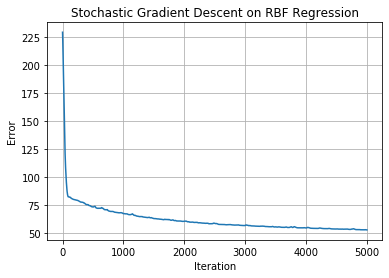
\includegraphics[width=1.0\textwidth]{rbf_sgd.png}
\captionof{figure}{Plot of the loss curves}
\end{minipage}

\subsection*{1.2 Mountain Car}

For the following tasks, a gaussian RBF is used to approximate the action value function of a mountain car problem using OpenAI Gym environment.
The goal of this problem is to get the under-power car to the top of the mountain.
The states consisted of 2D continuous values of position (-1.2 to 0.6) and velocity (-0.07 to 0.07), 
and the available actions are move left (0), no movement (1) and move right (2). 
For each time step, there is a reward (penalty) of -1 until the goal is reached.
This is a control problem where the agent needs to iteratively improve its policy in order to achieve its goal.
\vspace{-1em}
\subsection*{1.2.1 RBF Approximator from Tabular Discretization Method}

In this task, the mountain car is solved using Q-learning and tabular discretization method. 
The discretization of states is done by dividing the state space into 40 by 40 grids (velocity and position). 
In order to ensure that the agent can find optimal policy, extensive exploration of the state is needed.
Therefore, epsilon-greedy approach (with epsilon of 0.05) is used to select the next action.
Then, Q-learning, an off-policy model-free control algorithm, is applied to iteratively improve the action value table.
For this method, in the initial episode, it took more than thousands steps (achieving rewards of less than -1000s), 
and then gradually improve to achieve the rewards of around -200 in the 1000th episode. 

The next task is to use a gaussian RBF to approximate the action value function obtain from the above method, 
and determine if the policy obtained from the approximation is capable of driving the car to the top of the mountain.
The steps to use a gaussian RBF for function approximation are summarised as follows.

\vspace{-1em}
\begin{myitemize}
  \item The 3D Q tables are converted into 2D matrix where the columns consisted of position, velocity, action, and Q value.
        This process makes the data applicable for training where the position, velocity and action become the features, 
        and Q value becomes the target for regression.
  \item The number of basis functions, center and width of each basis function are selected the same way as mentioned in section 1.1.
  \item The optimisation is done in closed-form using Pseudo-inverse method to find the best weight ($w$).
\end{myitemize}    
\vspace{-1em}
Table \ref{rbf-accuracy} summarised the performance of an RBF model for value function approximator using different number of basis functions.
As shown in the table, the policy derived from an RBF with 100 and 200 basis functions were unable to drive the car to the top of the mountain.
In addition, the loss keeps decreasing with higher number of basis functions.
However, the average reward achieved from RBF with 400 basis functions is less than an RBF with 300 basis functions.
This could be due to the problem of overfitting where the model with too many basis functions overfit the discretized state features (the interpolation becomes less effective).

\begin{table}[htb]
  \centering
  \begin{tabular}{l p{1.2cm} p{3cm} p{3cm}}
  \toprule
     No. of Basis Functions & Loss & Goal Achieved & Ave. Reward\\ \midrule
  100 & 365.66 & No & None    \\ 
  200 & 323.40 & No & None   \\ 
  300 & 302.54 & Yes & -118.19   \\ 
  400 & 290.08 & Yes & -131.41   \\ 
  \bottomrule
\end{tabular}
\caption{Comparison of performance between different number of basis functions}
\label{rbf-accuracy}
\end{table}

\subsection*{1.2.2 Online Learning using Q and SARSA Update Rule}

Instead of using the obtained Q table to learn the weights of an RBF, they can be learned online using SGD with SARSA or Q-learning update rule.
Compare to the previous approach, we can use the raw continuous states without making them discrete, 
which will be beneficial for problems where the state space are large. 
In addition, learning online with function approximation also helps generalize the model for unseen states.
The process to learn the weight of RBF, as an action value function approximator, online can be summarised as follows.

\begin{myitemize}
  \item To generate the initial data for finding the hyperparameters for Gaussian RBF, such as the center and the width, 
  the state space are sampled randomly for 10000 data points.
  \item The sampled data are normalized to zero mean and unit variance.
  \item Using the sampled data, the number of basis functions, center and width of each basis function are selected the same way as mentioned in section 1.1.
  \item The RBF models are created based on the number of action (action-out approach), which means action are not part of the features.
  So for a mountain car problem, there will be a total of three RBF models, one for each action.
  \item The next action is selected based on epsilon-greedy policy (with epsilon = 0.05).
  \item For each time step, the weights of the RBF are updated using SGD with SARSA/ Q update rule.
\end{myitemize}  

Figure \ref{episode-reward} shows the reward of each episode over time using Q-learning update rule
with 200 basis functions, fixed learning rate of 0.01 and discount factor of 0.99. 
As shown in figure \ref{episode-reward}, the reward converges to around -130 after just 5 episode.
With better tuning of hyperparameters, such as learning rate, discount factor, and epsilon, 
the average reward would definitely increase further. 
Figure \ref{value-plot} shows the 3D plot of the value of the state space. 
For each state the value is calculated using the maximum value from all the actions from the approximated action value function.
As expected, the value is high on the top right of the figure, which is where the position is near the goal and the velocity is high.

\begin{figure}[h]
  \centering
  \begin{minipage}{0.45\textwidth}
      \centering
      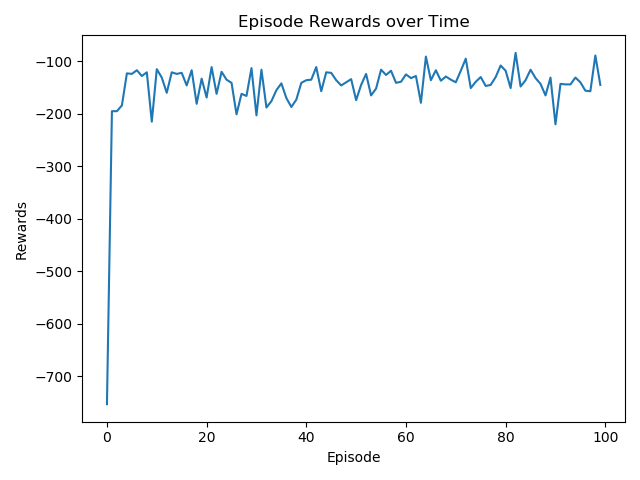
\includegraphics[width=0.9\textwidth]{q-online.png} % first figure itself
      \caption{Episode reward over time}
      \label{episode-reward}
  \end{minipage}\hfill
  \begin{minipage}{0.55\textwidth}
      \centering
      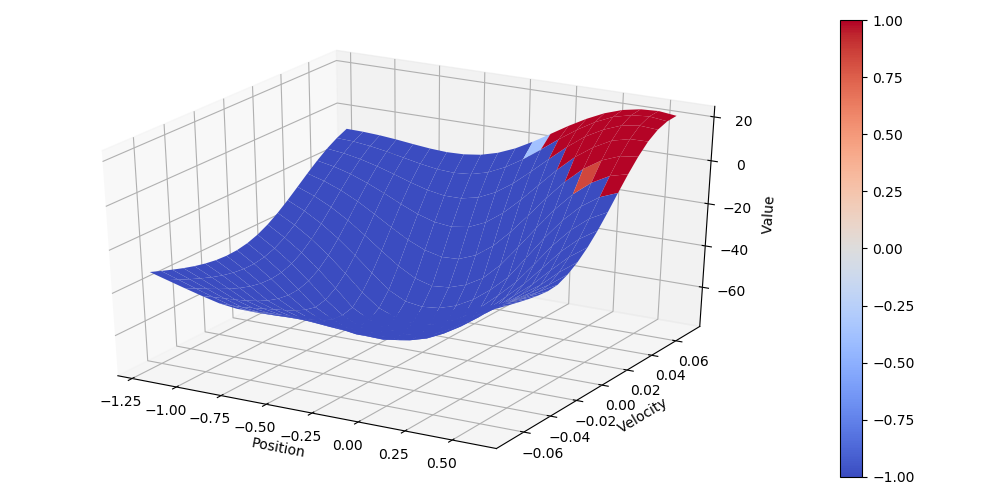
\includegraphics[width=1\textwidth]{mountain-value.png} % second figure itself
      \caption{3D plot of the value function after 1000 episodes}
      \label{value-plot}
  \end{minipage}
\end{figure}

\newpage
Snippet of code of an RL agent using gaussian RBF as an action value function approximator.
\begin{lstlisting}[language=Python]
# generate basis function center using K-means clustering and sampled environment states.
def init_rbf(self, env, n_basis=100):
    observation_examples = np.array([env.observation_space.sample() for x in range(10000)])
    scaler = StandardScaler()
    scaler.fit(observation_examples)
    scaled_examples = scaler.transform(observation_examples)
    kmeans = KMeans(n_clusters=n_basis, random_state=0).fit(scaled_examples)
    return kmeans.cluster_centers_

# get Q value from a given state and action
def q(self, state, action):
    features = self.feature_transformer.featurize_state(state)
    return np.dot(features, self.w[action])

# given state choose next action based on epsilon greedy policy
def epsilon_greedy(self, state):
    y = self.predict(state)
    if np.random.uniform(low=0, high=1) < epsilon:
        chosen_action = env.action_space.sample()
    else:
        chosen_action = np.argmax(y)
    return chosen_action

# given state, predict value for all actions 
def predict(self, state):
    features = self.feature_transformer.featurize_state(state)
    return features @ self.w.T

# update the weight using SARSA update rule
def sarsa_update(self, lr, reward, gamma, state, action, next_state, next_action):
    feature = feature_transformer.featurize_state(state).flatten()
    self.w[action] += lr * (reward + gamma * self.q(next_state, next_action) - self.q(state, action)) * feature

# update the weight using Q-learning update rule
def q_update(self, lr, reward, gamma, state, action, next_state):
    feature = feature_transformer.featurize_state(state).flatten()
    next_q_max = np.max(self.predict(next_state))
    self.w[action] += lr * (reward + gamma * next_q_max - self.q(state, action)) * feature
  \end{lstlisting}

\subsection*{1.3 Resource Allocation Network}



\section*{Part 2: Summarising a Recent Scientific Study}

\subsection*{2.1 Human-level Control through Deep Reinforcement
Learning}



\end{document}
